\documentclass[tikz,border=8pt]{standalone}
\usetikzlibrary{arrows.meta,backgrounds,fit,positioning,shapes.geometric}

\definecolor{marletBlue}{HTML}{D8E8FF}
\definecolor{marletBlueBorder}{HTML}{3568A8}
\definecolor{marletGreen}{HTML}{DDF3E4}
\definecolor{marletGreenBorder}{HTML}{2D7A46}
\definecolor{marletGold}{HTML}{FFF0C2}
\definecolor{marletGoldBorder}{HTML}{A96C00}
\definecolor{marletRed}{HTML}{FFE0DE}
\definecolor{marletRedBorder}{HTML}{A9453D}
\definecolor{marletGray}{HTML}{F3F4F6}
\definecolor{marletGrayBorder}{HTML}{6B7280}
\definecolor{marletPurple}{HTML}{E8E1FF}
\definecolor{marletPurpleBorder}{HTML}{6650A4}

\begin{document}
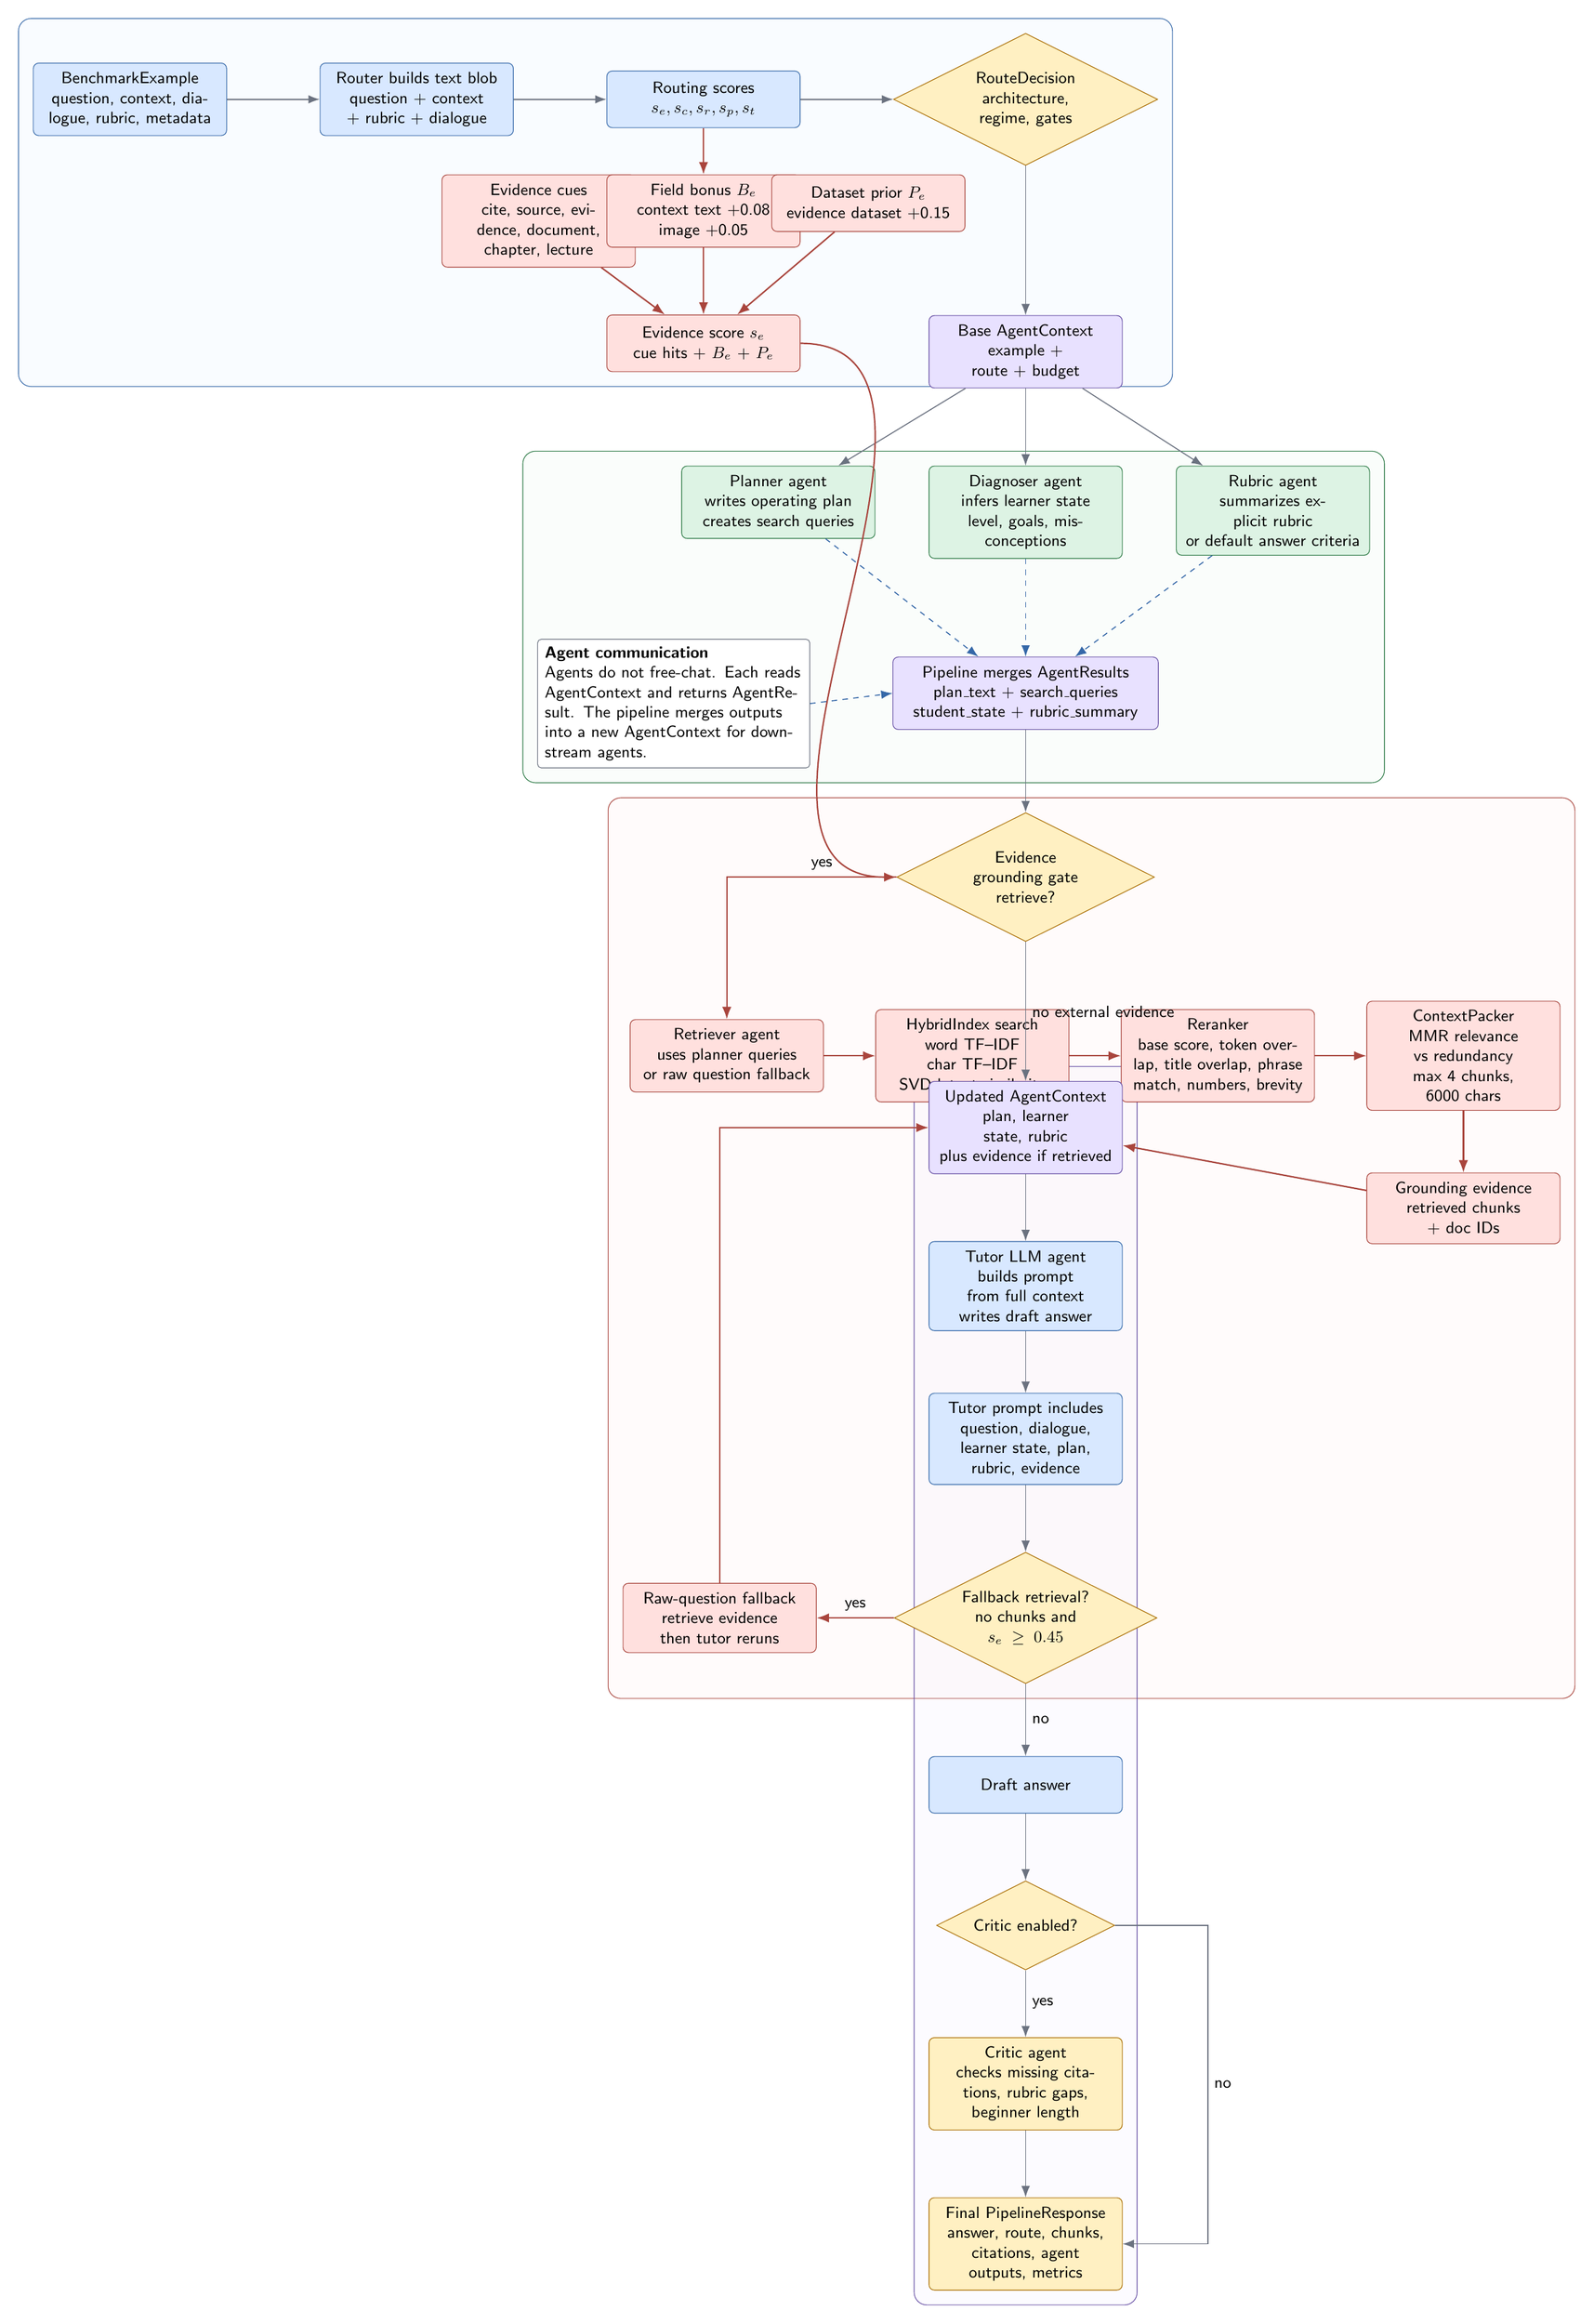
\begin{tikzpicture}[
  font=\sffamily\small,
  node distance=8mm and 12mm,
  >=Latex,
  flow/.style={-{Latex[length=2.2mm]}, line width=0.55pt, draw=marletGrayBorder},
  evidenceFlow/.style={-{Latex[length=2.4mm]}, line width=0.8pt, draw=marletRedBorder},
  dataFlow/.style={-{Latex[length=2.2mm]}, line width=0.55pt, draw=marletBlueBorder, dashed},
  box/.style={rectangle, rounded corners=3pt, draw=marletGrayBorder, fill=marletGray, align=center, inner sep=5pt, text width=34mm, minimum height=11mm},
  bluebox/.style={box, draw=marletBlueBorder, fill=marletBlue},
  greenbox/.style={box, draw=marletGreenBorder, fill=marletGreen},
  goldbox/.style={box, draw=marletGoldBorder, fill=marletGold},
  redbox/.style={box, draw=marletRedBorder, fill=marletRed},
  purplebox/.style={box, draw=marletPurpleBorder, fill=marletPurple},
  decision/.style={diamond, aspect=2.0, draw=marletGoldBorder, fill=marletGold, align=center, inner sep=1.5pt, text width=27mm},
  smallnote/.style={rectangle, rounded corners=2pt, draw=marletGrayBorder, fill=white, align=left, inner sep=4pt, text width=50mm}
]

% Top-level input and routing.
\node[bluebox] (input) {BenchmarkExample\\question, context, dialogue, rubric, metadata};
\node[bluebox, right=18mm of input] (blob) {Router builds text blob\\question + context + rubric + dialogue};
\node[bluebox, right=18mm of blob] (scores) {Routing scores\\$s_e,s_c,s_r,s_p,s_t$};
\node[decision, right=18mm of scores] (route) {RouteDecision\\architecture, regime, gates};

\draw[flow] (input) -- (blob);
\draw[flow] (blob) -- (scores);
\draw[flow] (scores) -- (route);

% Evidence score detail.
\node[redbox, below=9mm of scores, xshift=-32mm] (cue) {Evidence cues\\cite, source, evidence, document, chapter, lecture};
\node[redbox, below=9mm of scores] (bonus) {Field bonus $B_e$\\context text +0.08\\image +0.05};
\node[redbox, below=9mm of scores, xshift=32mm] (prior) {Dataset prior $P_e$\\evidence dataset +0.15};
\node[redbox, below=13mm of bonus] (evidenceScore) {Evidence score $s_e$\\cue hits + $B_e$ + $P_e$};

\draw[evidenceFlow] (cue) -- (evidenceScore);
\draw[evidenceFlow] (bonus) -- (evidenceScore);
\draw[evidenceFlow] (prior) -- (evidenceScore);
\draw[evidenceFlow] (scores) -- (bonus);

% Pipeline start.
\node[purplebox, below=29mm of route] (baseContext) {Base AgentContext\\example + route + budget};
\draw[flow] (route) -- (baseContext);

% Parallel specialists.
\node[greenbox, below=15mm of baseContext, xshift=-48mm] (planner) {Planner agent\\writes operating plan\\creates search queries};
\node[greenbox, below=15mm of baseContext] (diagnoser) {Diagnoser agent\\infers learner state\\level, goals, misconceptions};
\node[greenbox, below=15mm of baseContext, xshift=48mm] (rubric) {Rubric agent\\summarizes explicit rubric\\or default answer criteria};

\draw[flow] (baseContext) -- (planner);
\draw[flow] (baseContext) -- (diagnoser);
\draw[flow] (baseContext) -- (rubric);

\node[purplebox, below=19mm of diagnoser, text width=48mm] (merge) {Pipeline merges AgentResults\\plan\_text + search\_queries\\student\_state + rubric\_summary};
\draw[dataFlow] (planner) -- (merge);
\draw[dataFlow] (diagnoser) -- (merge);
\draw[dataFlow] (rubric) -- (merge);

% Retrieval gate and evidence path.
\node[decision, below=16mm of merge] (gate) {Evidence grounding gate\\retrieve?};
\draw[flow] (merge) -- (gate);
\draw[evidenceFlow] (evidenceScore.east) to[out=0,in=180] (gate.west);

\node[redbox, below=15mm of gate, xshift=-58mm] (retriever) {Retriever agent\\uses planner queries\\or raw question fallback};
\node[redbox, right=10mm of retriever] (index) {HybridIndex search\\word TF--IDF\\char TF--IDF\\SVD latent similarity};
\node[redbox, right=10mm of index] (rerank) {Reranker\\base score, token overlap, title overlap, phrase match, numbers, brevity};
\node[redbox, right=10mm of rerank] (pack) {ContextPacker\\MMR relevance vs redundancy\\max 4 chunks, 6000 chars};
\node[redbox, below=12mm of pack] (chunks) {Grounding evidence\\retrieved chunks + doc IDs};

\draw[evidenceFlow] (gate) -| node[pos=0.22, above, sloped] {yes} (retriever);
\draw[evidenceFlow] (retriever) -- (index);
\draw[evidenceFlow] (index) -- (rerank);
\draw[evidenceFlow] (rerank) -- (pack);
\draw[evidenceFlow] (pack) -- (chunks);

% Tutor path.
\node[purplebox, below=27mm of gate] (tutorContext) {Updated AgentContext\\plan, learner state, rubric\\plus evidence if retrieved};
\draw[flow] (gate) -- node[right] {no external evidence} (tutorContext);
\draw[evidenceFlow] (chunks) -- (tutorContext);

\node[bluebox, below=13mm of tutorContext] (tutor) {Tutor LLM agent\\builds prompt from full context\\writes draft answer};
\node[bluebox, below=12mm of tutor] (prompt) {Tutor prompt includes\\question, dialogue, learner state, plan, rubric, evidence};
\draw[flow] (tutorContext) -- (tutor);
\draw[flow] (tutor) -- (prompt);

% Fallback and critic.
\node[decision, below=13mm of prompt] (fallback) {Fallback retrieval?\\no chunks and $s_e \ge 0.45$};
\node[redbox, left=15mm of fallback] (fallbackRetrieval) {Raw-question fallback\\retrieve evidence\\then tutor reruns};
\node[bluebox, below=14mm of fallback] (draft) {Draft answer};
\draw[flow] (prompt) -- (fallback);
\draw[evidenceFlow] (fallback) -- node[above] {yes} (fallbackRetrieval);
\draw[evidenceFlow] (fallbackRetrieval) |- (tutorContext);
\draw[flow] (fallback) -- node[right] {no} (draft);

\node[decision, below=13mm of draft] (criticGate) {Critic enabled?};
\node[goldbox, below=13mm of criticGate] (critic) {Critic agent\\checks missing citations, rubric gaps, beginner length};
\node[goldbox, below=13mm of critic] (final) {Final PipelineResponse\\answer, route, chunks, citations, agent outputs, metrics};
\draw[flow] (draft) -- (criticGate);
\draw[flow] (criticGate) -- node[right] {yes} (critic);
\draw[flow] (critic) -- (final);
\draw[flow] (criticGate.east) -- ++(18mm,0) |- node[pos=0.25, right] {no} (final.east);

% Communication note.
\node[smallnote, left=16mm of merge, yshift=-2mm] (comm) {\textbf{Agent communication}\\Agents do not free-chat. Each reads AgentContext and returns AgentResult. The pipeline merges outputs into a new AgentContext for downstream agents.};
\draw[dataFlow] (comm.east) -- (merge.west);

% Background groups.
\begin{scope}[on background layer]
  \node[draw=marletBlueBorder, fill=marletBlue, fill opacity=0.14, rounded corners=7pt, fit=(input)(blob)(scores)(route)(cue)(bonus)(prior)(evidenceScore), inner sep=8pt] {};
  \node[draw=marletGreenBorder, fill=marletGreen, fill opacity=0.16, rounded corners=7pt, fit=(planner)(diagnoser)(rubric)(merge)(comm), inner sep=8pt] {};
  \node[draw=marletRedBorder, fill=marletRed, fill opacity=0.13, rounded corners=7pt, fit=(gate)(retriever)(index)(rerank)(pack)(chunks)(fallback)(fallbackRetrieval), inner sep=8pt] {};
  \node[draw=marletPurpleBorder, fill=marletPurple, fill opacity=0.12, rounded corners=7pt, fit=(tutorContext)(tutor)(prompt)(draft)(criticGate)(critic)(final), inner sep=8pt] {};
\end{scope}

\end{tikzpicture}
\end{document}
